\subsection{Long-baseline neutrino beams }

Neutrino beams~\cite{Kopp2007101} based on particle accelerators have been used since the 1960s, when they provided the evidence for the existence of two types of neutrino, $\nu_e$ and $\nu_\mu$. The general design is based on a high intensity proton beam impinging on a target and producing pions and kaons through interactions on the target nuclei. 
These mesons decay in a dedicated volume downstream of the target, creating mainly a $\nu_\mu$ beam.  

The long baseline beams are based on the so called wide band beam concept. Here the secondary charged mesons are focused using a system of magnetic devices, called horns. The horns, usually with a cylindrical symmetry around the beam, are pulsed with a very intense current in coincidence with the arrival of the beam. 
%The ratio between the primary proton energy and the typical neutrino energy is %at least a factor ten, and the neutrino spectrum extends for about a decade %around this typical energy.  

The flux is tuned in such a way that the phase $\Delta m^2_{32} L/ (4 E)$ reaches $\pi/2$ for the design baseline $L$ and the peak energy $E$, in order to probe the atmospheric oscillation sector with the beam $\nu_\mu$. To do so, the proton energy, the target length and width, the focussing system and the decay volume length and width need to be accurately designed and optimized.   

An off-axis neutrino beam \cite{1995bnl} relies on the following idea: as the $\nu_\mu$ are mainly produced by the two-body decays of pions, there is a correlation between pion energy $E_\pi$, the neutrino energy $E_\nu$ and the decay angle $\theta$ 
\begin{equation}
E_\nu = \frac{(1-(m_\mu/m_\pi)^2) E_\pi}{(1+\gamma^2 \theta^2) } 
\end{equation}
valid in the limit of small angles.

Neutrinos emitted at a small angle with respect to the pion direction have a distinct narrow spectrum peaking at a much lower energy with respect to the on axis beam. This feature that has been used by the T2K and NOvA experiments, offers several advantages because it avoids the large high energy tail of the on axis beam, thereby reducing some background reactions. 

\begin{figure}[htbp]
\centering
%\includegraphics[width=0.5\linewidth]{energy_miniboone.eps}
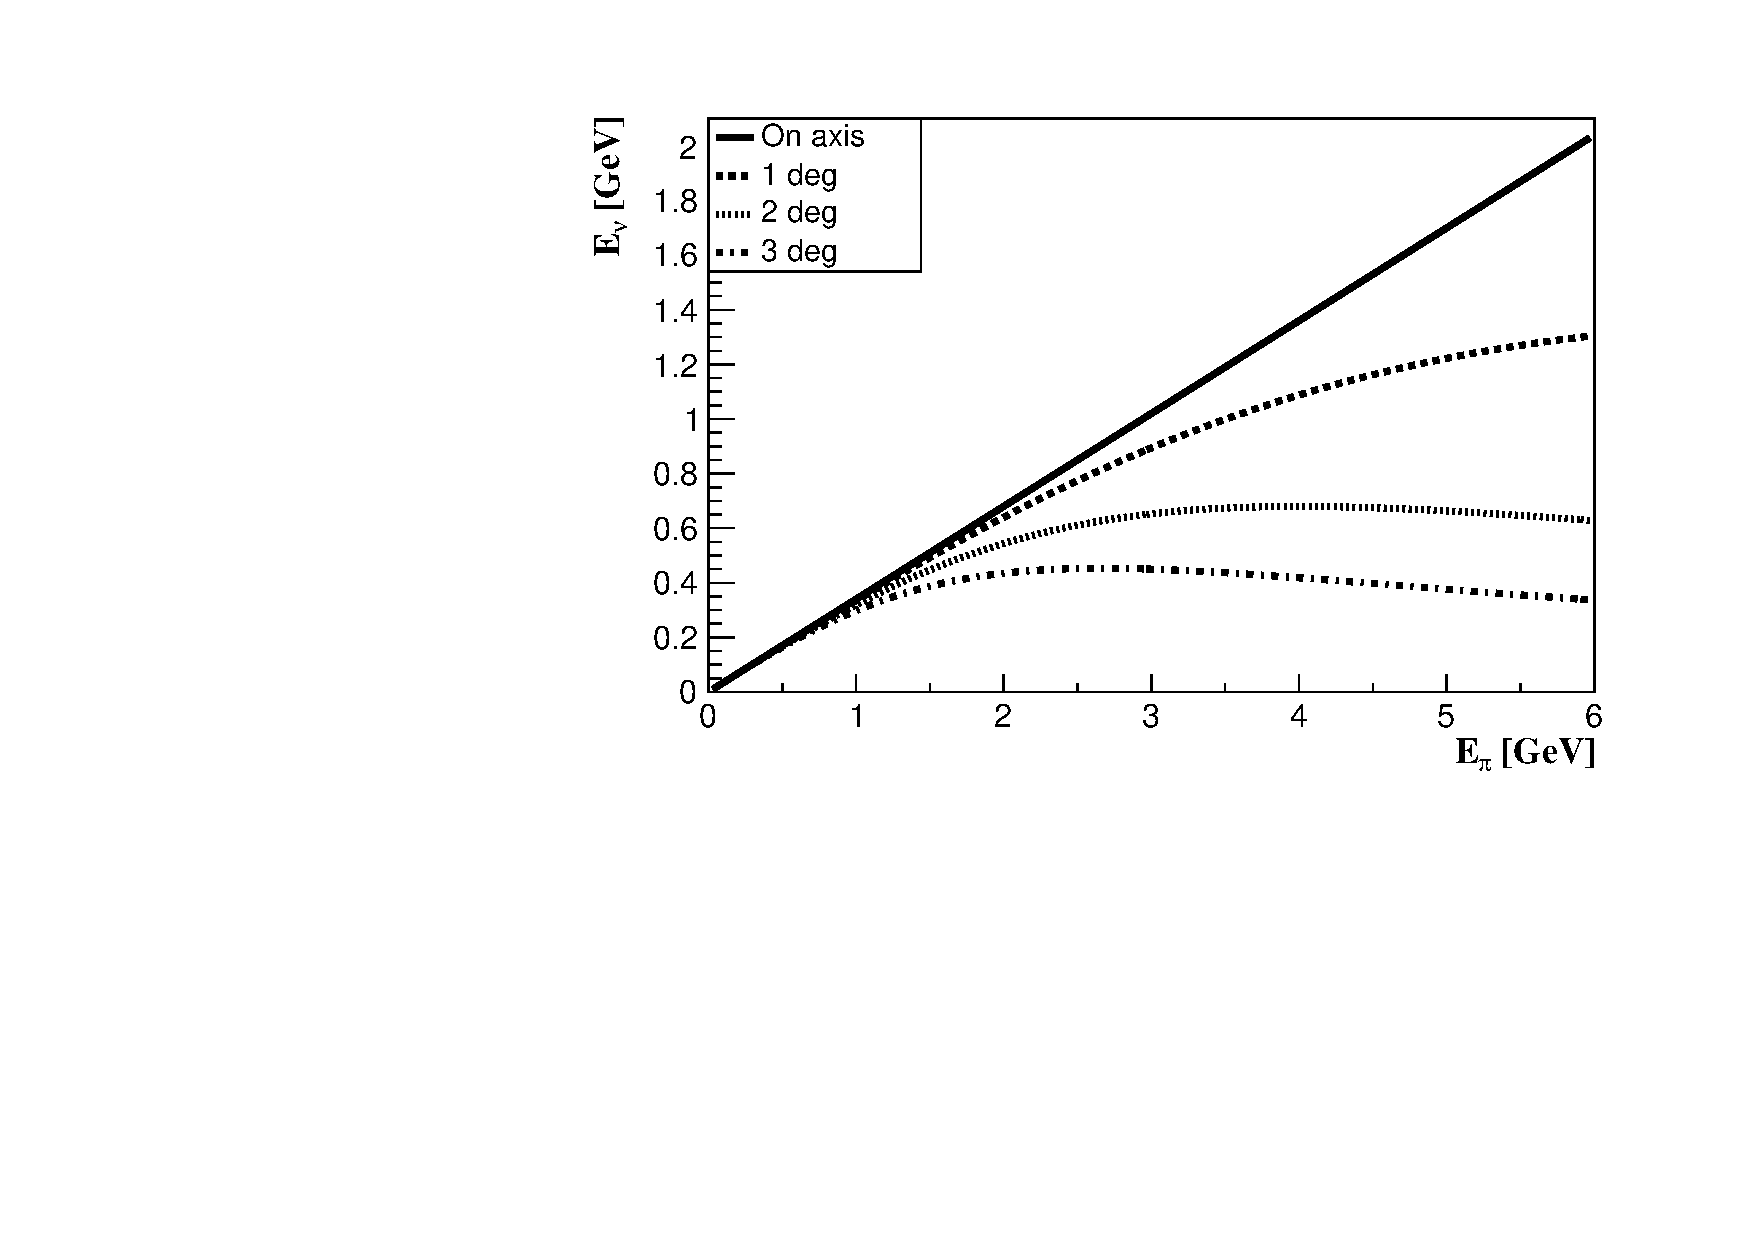
\includegraphics[width=0.6\linewidth]{figures/offaxis.pdf}
  \caption{Neutrino energy as a function of the pion energy for on-axis decays and several off-axis angles. For a non-zero off-axis angle, the neutrino energy reaches a maximum. This feature is currently exploited in the T2K and NOvA experiments.}
 \label{fig:offaxis}
 \end{figure}


As the neutrino beam is a tertiary beam, it is necessary to include in the experimental apparatus monitoring devices to ensure that it is stable in intensity and direction. To this effect, muon detectors, sensitive to the muons produced by the pion decays, are placed close to the end of the decay volume. Moreover, as the neutrino flux and cross-sections and the beam composition are not known with sufficient precision, a near detector is located close to the target station (typically within a few hundred meters). The near detector constrains the neutrino interaction rate, proportional to the product t=of neutrino flux and the cross-section. Moreover, the near detector allows to measure the beam composition and to perform study of several neutrino cross-section.    

Description of T2K beam line if space allows.

\begin{table}
\centering
\begin{tabular}{|c|c|c|c|c|c|}
  \hline
  Exp. & Energy (GeV) & Power (kW) & L (km) & FD mass (kt) & POT \\ 
  \hline
K2K & 30 & & 250 & 22.5 & \\
MINOS & 120 & 700 & 790 & 5.4 &\\
OPERA & 450 & 732 &  & & 1.8 10$^{20}$\\
T2K & 30 & 750 & 295 & 22.5 & 8 10$^{21}$\\
NOvA & 120 & 700& 810 & 14 & \\
HK & 30 & & & & \\
DUNE & 120 & 1200 & 1300 & 40 &\\
  \hline
\end{tabular}
\caption{Parameters of recent and future long baseline experiments. Energy and power refer to the primary proton beam, L is the baseline, FD the mass of the far detector. POT (Proton On Target) represents the integrated dataset as of 2016.}
\end{table}


\subsubsection{Results from long-baseline accelerator experiments K2K MINOS T2K NOVA}

K2K (KEK-to-Kamioka) was the first long baseline neutrino beam, using Super-Kamiokande as its far detector at 290 km from the neutrino production. Operating between 1999 and 2004, it has measured the disappearance of $\nu_\mu$: 112 events were observed, while 158.1$^{+9.2}_{-8.6}$ were expected without oscillation, a 4.3 $\sigma$ effect~\cite{Ahn:2006zza}. This measurement has confirmed neutrino oscillation as the explanation for the atmospheric neutrino disappearance. 

Further precision measurements of the $\nu_\mu \rightarrow \nu_\mu$ were reported by MINOS, T2K and NOvA.

We will here describe in some detail the T2K measurement, the most precise for what concerns the $\theta_{23}$ angle.

\begin{figure}[htbp]
\centering
%\includegraphics[width=0.5\linewidth]{energy_miniboone.eps}
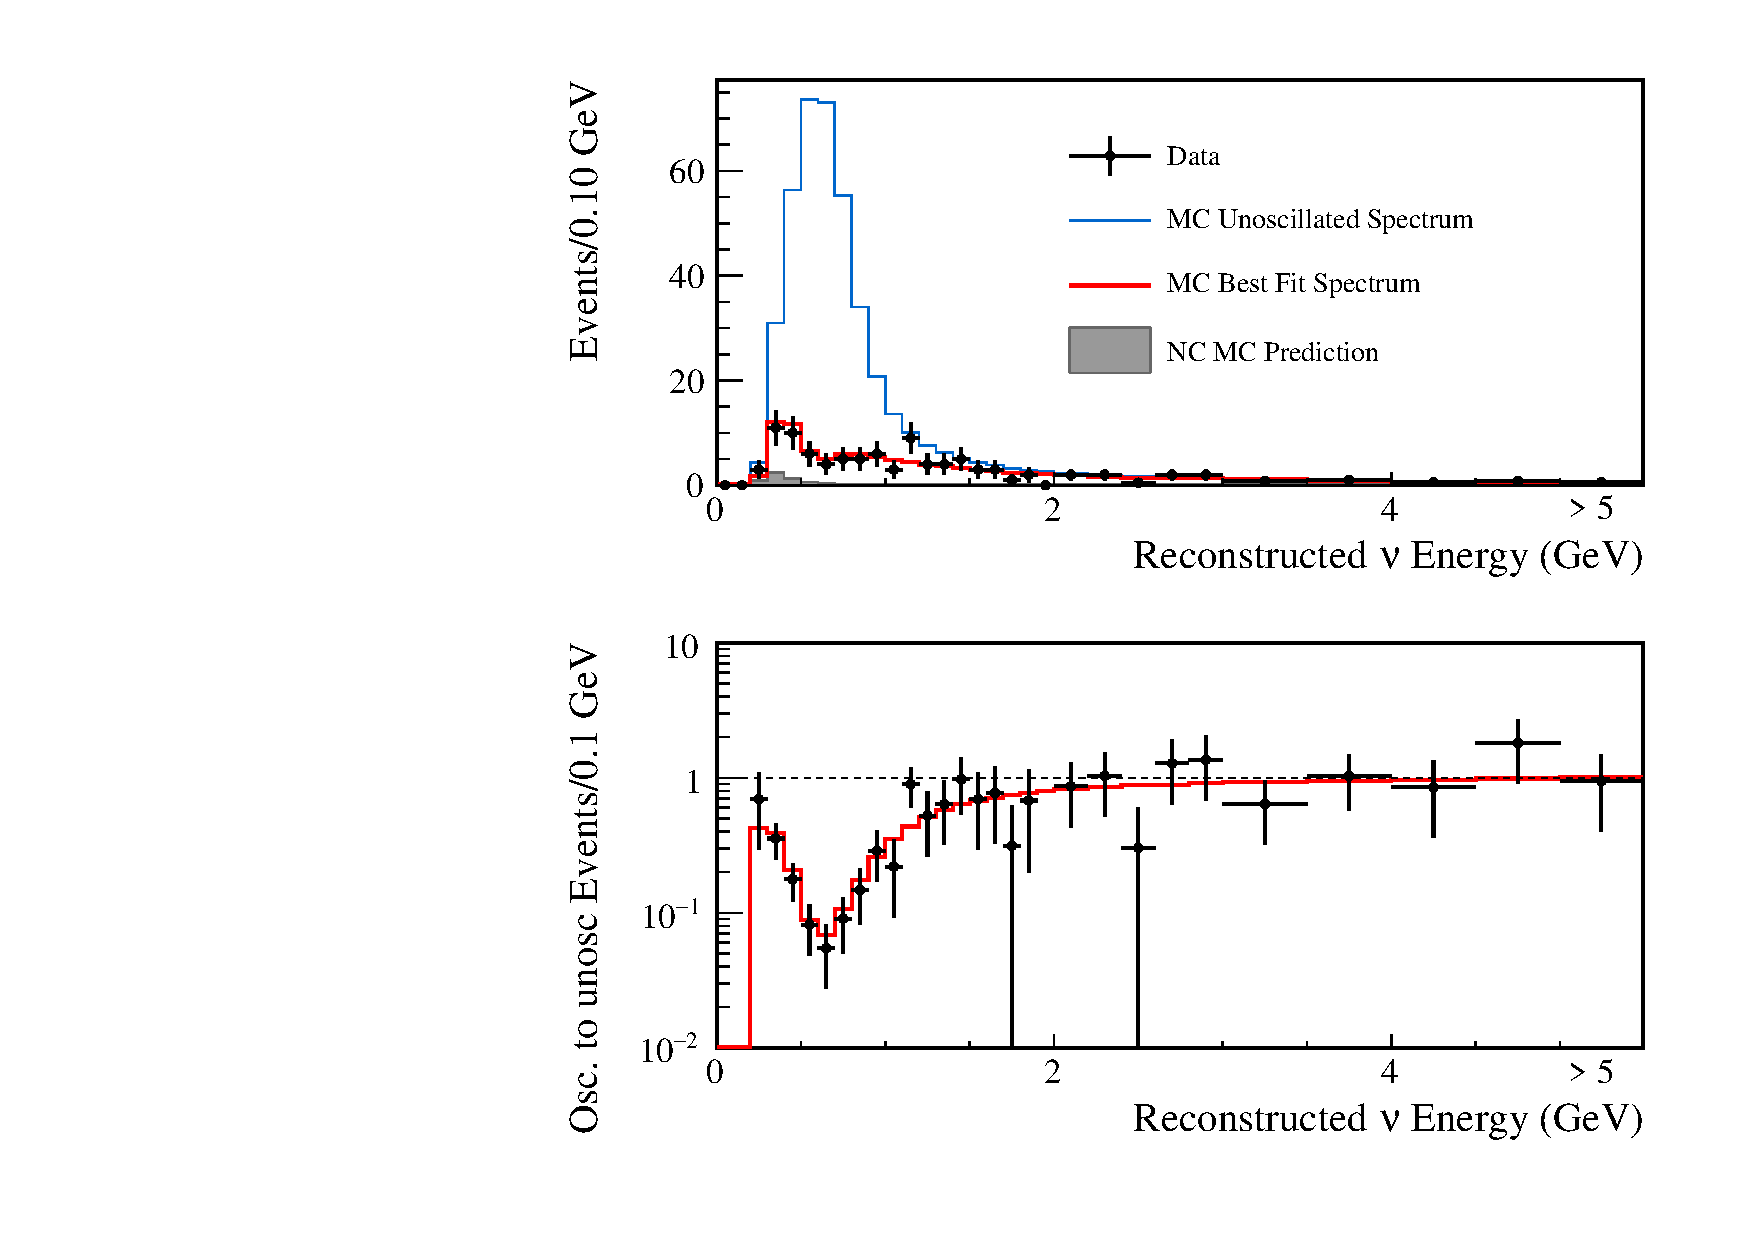
\includegraphics[width=0.6\linewidth]{figures/t2k-disapp.pdf}
  \caption{
Reconstructed $\nu_\mu$ energy spectrum by the T2K collaboration for data, best-fit prediction, and
unoscillated prediction. Bottom: Ratio of oscillated to unoscillated events as a function of
neutrino energy for the data and the best-fit spectrum.
}
 \label{fig:t2kdis}
 \end{figure}

\begin{figure}[htbp]
\centering
%\includegraphics[width=0.5\linewidth]{energy_miniboone.eps}
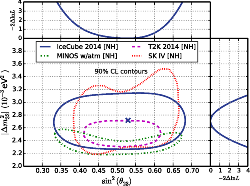
\includegraphics[width=0.6\linewidth]{figures/atm-contour.pdf}
  \caption{
  90\% CL regions in the plane $\Delta m^2 $ versus $\sin^2 (2 \theta_{23}$
  determined by Super-Kamiokande and IceCube-DeepCore using atmospheric neutrinos, and MINOS and T2K using long baseline neutrino beams. 
}
 \label{fig:atm-contour}
 \end{figure}
 
 
 \subsubsection{Evidence for $\nu_\tau$ appearance}

The OPERA experiment on the CERN to Gran Sasso neutrino beam, taking data between 2008 and 2012, was designed to test the $\nu_\mu \rightarrow \nu_\tau$ appearance hypothesis. The detector is based on the Emulsion Cloud Chamber technique, with 1800 ton of nuclear emulsion detectors in the forms of bricks, each brick being composed of a stack of nuclear emulsion film and lead plates. This target, capable of sub-micrometric track resolution, is devoted to the study of the neutrino interaction vertex and the particles associated to it. The identification of the $\tau$ leptons relies mainly on their characteristic kink (Fig.~\ref{fig:opera}) due to the decay $\tau \rightarrow h \nu_\tau$, or $\tau \rightarrow l \nu_\tau \bar \nu_l$, where $h$ is a charged meson, and $l$ is an electron or a muon. Another signature is related to the decay $\tau \rightarrow 3 h \nu_\tau$ where the short $\tau$ track ends in a three-pronged vertex. The target detectors are complemented by scintillator trackers and muon spectrometers. 

OPERA has observed 5 $\nu_\tau$ candidate events \cite{Agafonova:2015jxn} with a total background of 
$0.25 \pm 0.05$ events, mainly coming from decays of charmed particles. This corresponds to a 5.1 $\sigma$ observation of $\nu_\tau$ production in an oscillated $\nu_\mu$ beam. 

The Super-Kamiokande collaboration has also searched for $\nu_\tau$ appearance in multi-ring events to test the hypothesis of $\nu_\mu \rightarrow \nu_\tau$ oscillations~\cite{Abe:2012jj}. While the selected sample is affected by large backgrounds, there is an excess of tau-like events in the upward-going direction with a significance of 3.8 $\sigma$, offering a complementary confirmation of the OPERA result.  
 
\begin{figure}[htbp]
\centering
%\includegraphics[width=0.5\linewidth]{energy_miniboone.eps}
%\includegraphics[width=0.6\linewidth]{figures/topology_modified.pdf}
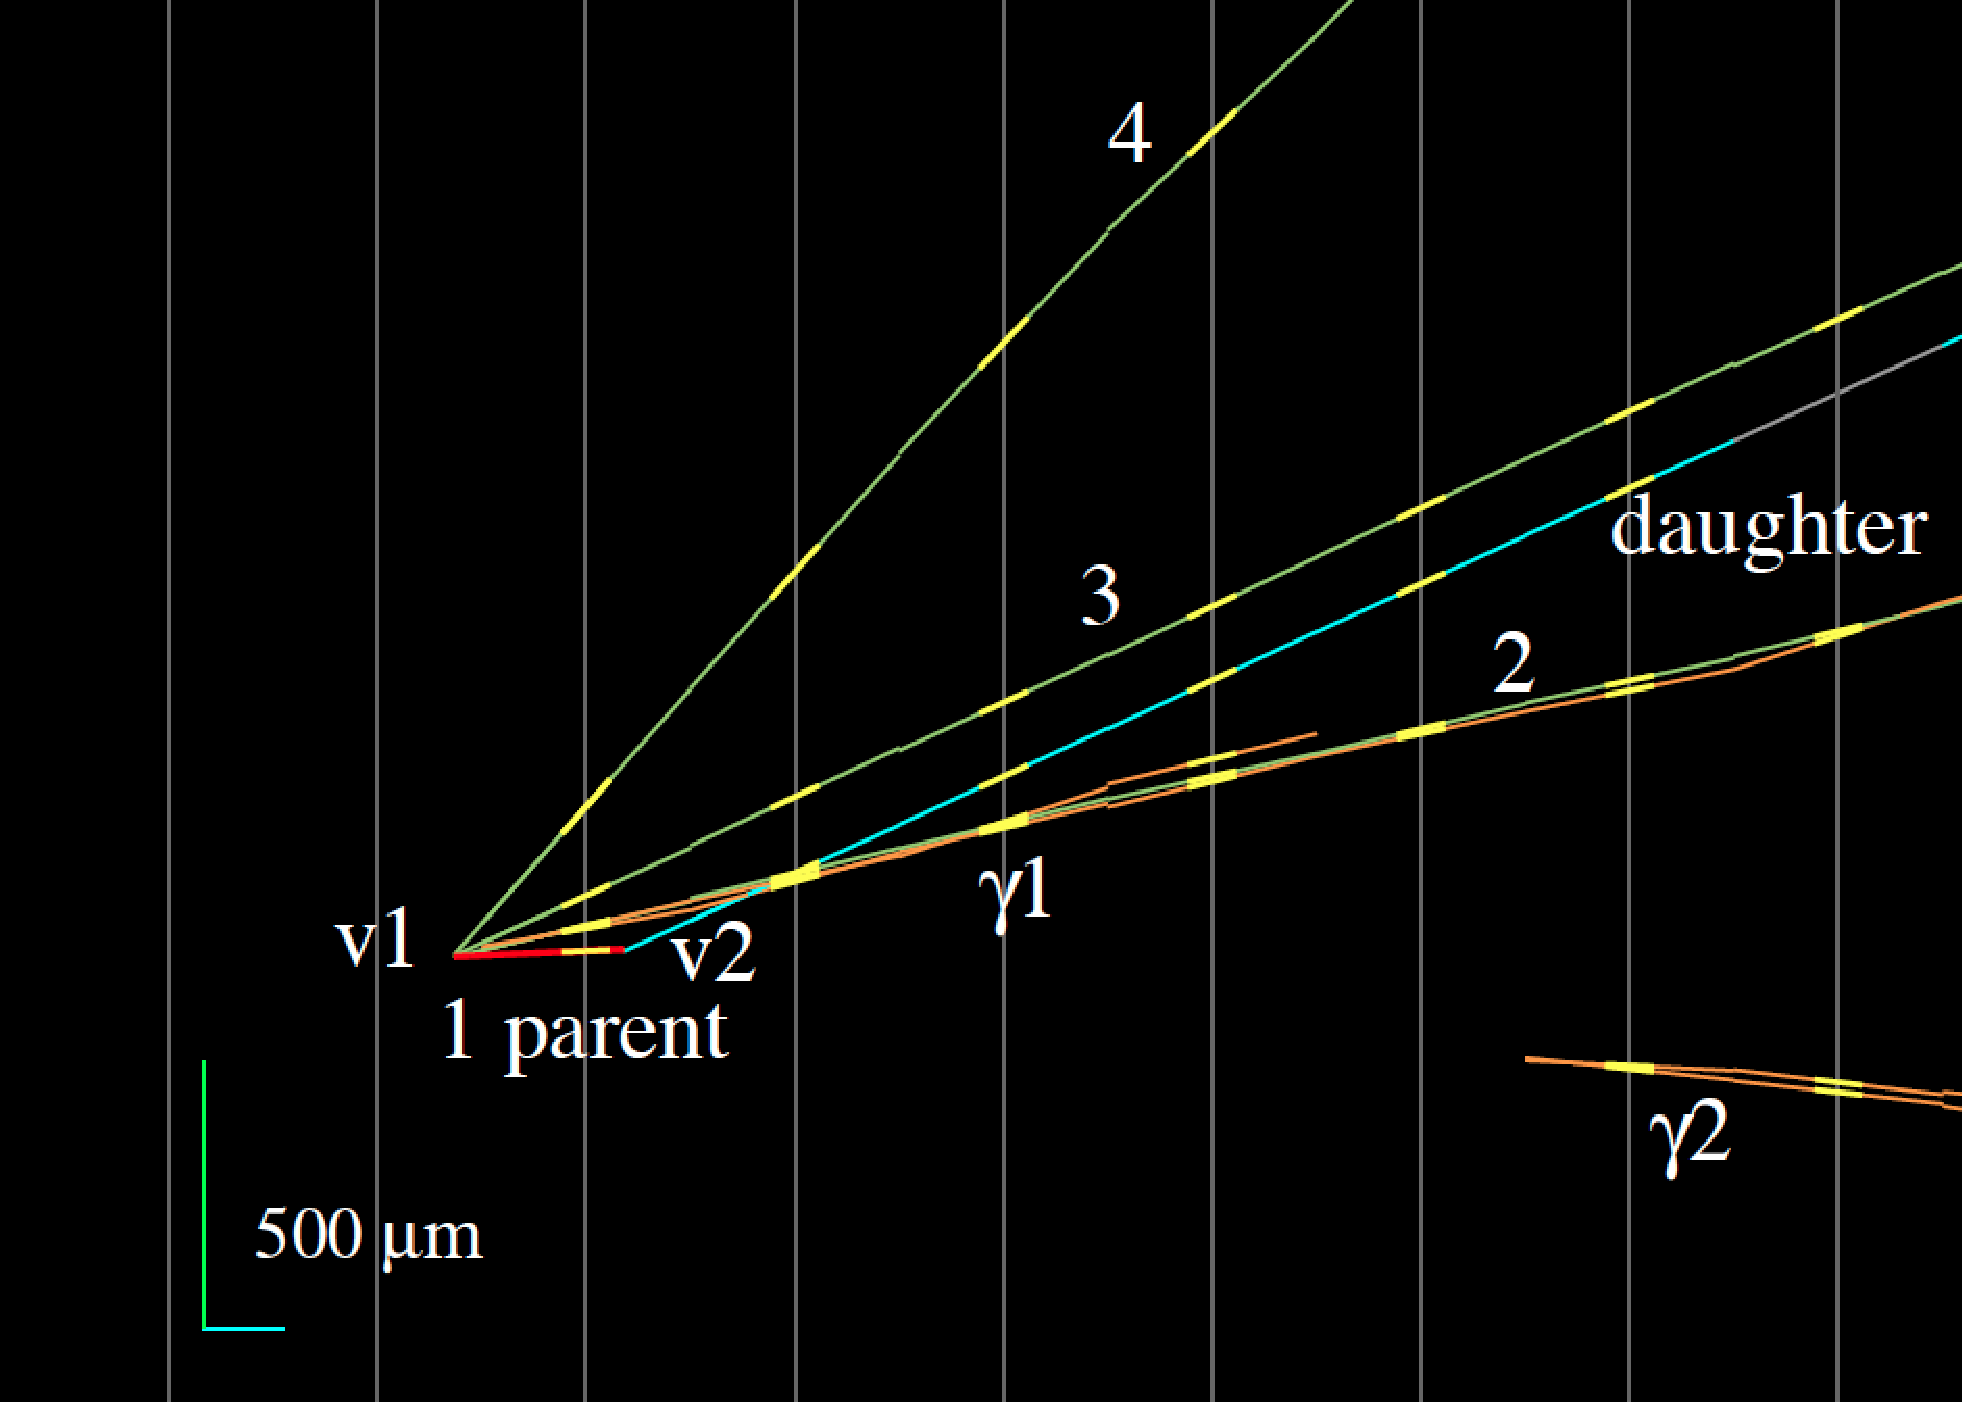
\includegraphics[width=0.6\linewidth]{figures/tau4.pdf}
  \caption{
Event display of the fourth $\nu_\tau$ candidate event from the OPERA 
experiment~\cite{DICRESCENZO2015186} in the
horizontal projection longitudinal to the neutrino direction.
The primary and secondary vertices are indicated as V$_0$ and
V$_1$ , respectively. The kink between the parent and daughter track, a feature of $\tau$ lepton decays, is clearly visible. The yellow stubs represent the track segments as measured in the emulsion films.  
}
 \label{fig:opera}
 \end{figure}

